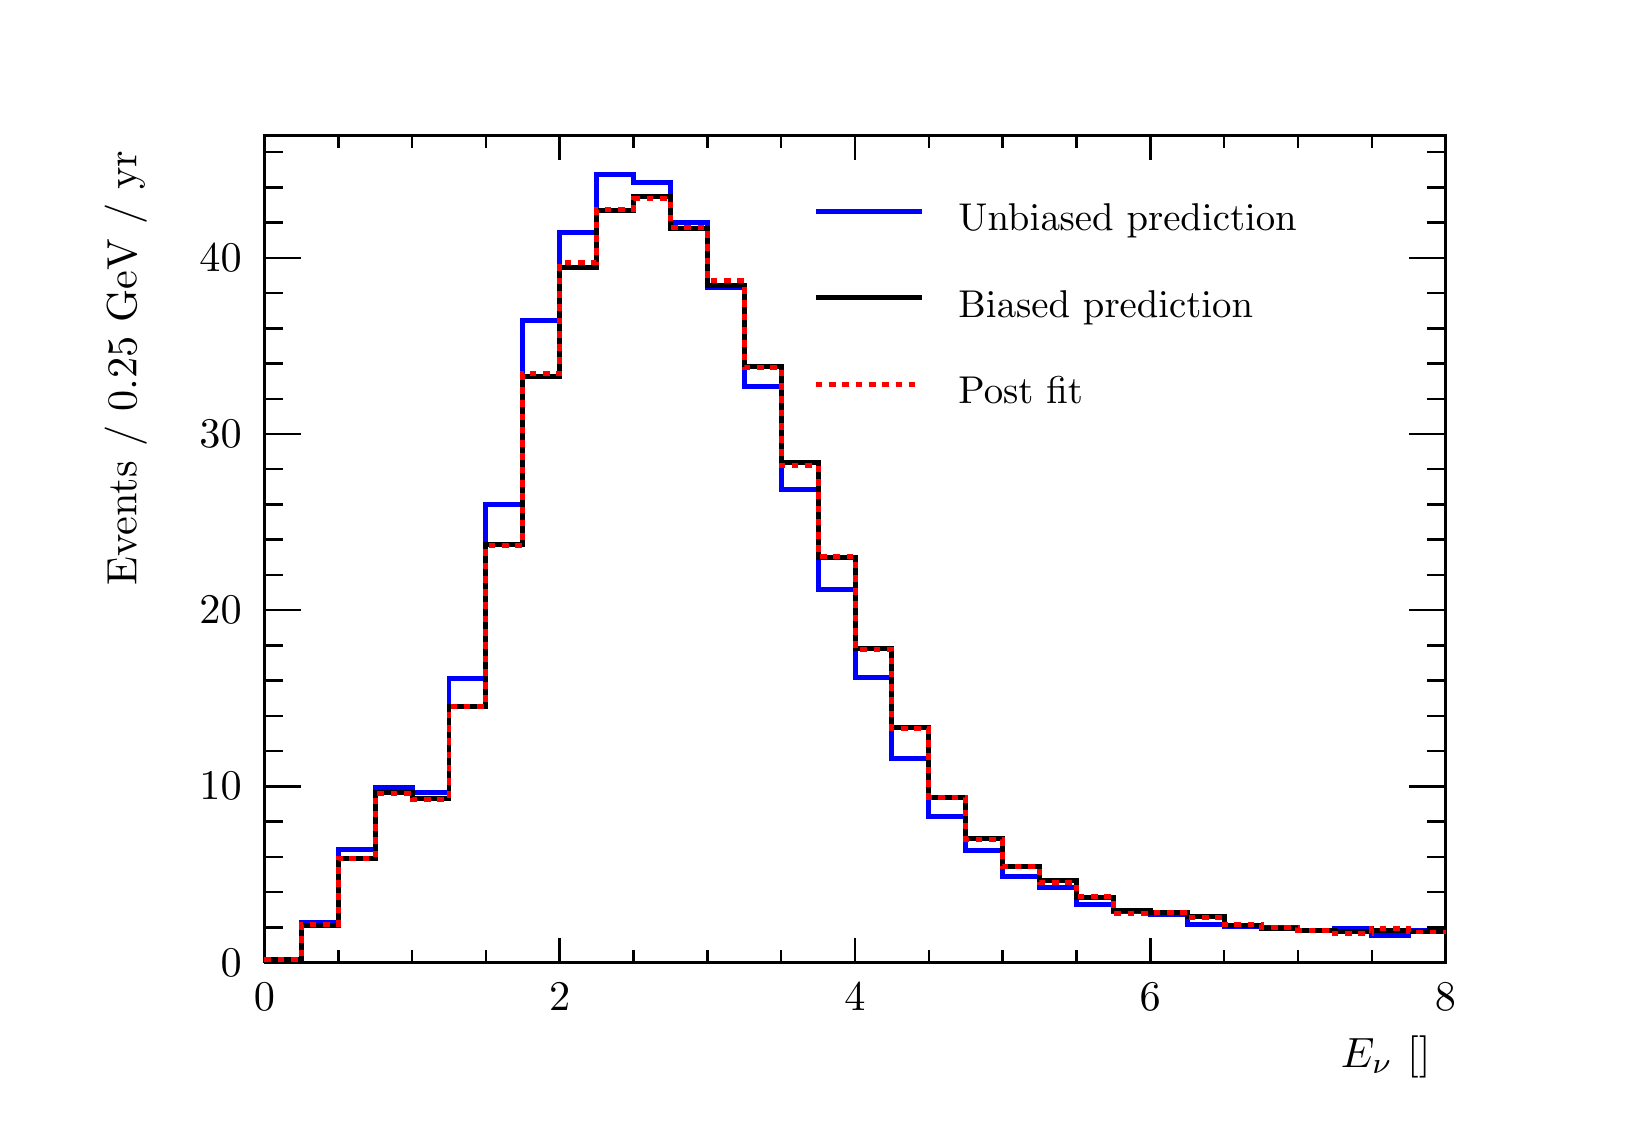
\begin{tikzpicture}
\pgfdeclareplotmark{cross} {
\pgfpathmoveto{\pgfpoint{-0.3\pgfplotmarksize}{\pgfplotmarksize}}
\pgfpathlineto{\pgfpoint{+0.3\pgfplotmarksize}{\pgfplotmarksize}}
\pgfpathlineto{\pgfpoint{+0.3\pgfplotmarksize}{0.3\pgfplotmarksize}}
\pgfpathlineto{\pgfpoint{+1\pgfplotmarksize}{0.3\pgfplotmarksize}}
\pgfpathlineto{\pgfpoint{+1\pgfplotmarksize}{-0.3\pgfplotmarksize}}
\pgfpathlineto{\pgfpoint{+0.3\pgfplotmarksize}{-0.3\pgfplotmarksize}}
\pgfpathlineto{\pgfpoint{+0.3\pgfplotmarksize}{-1.\pgfplotmarksize}}
\pgfpathlineto{\pgfpoint{-0.3\pgfplotmarksize}{-1.\pgfplotmarksize}}
\pgfpathlineto{\pgfpoint{-0.3\pgfplotmarksize}{-0.3\pgfplotmarksize}}
\pgfpathlineto{\pgfpoint{-1.\pgfplotmarksize}{-0.3\pgfplotmarksize}}
\pgfpathlineto{\pgfpoint{-1.\pgfplotmarksize}{0.3\pgfplotmarksize}}
\pgfpathlineto{\pgfpoint{-0.3\pgfplotmarksize}{0.3\pgfplotmarksize}}
\pgfpathclose
\pgfusepathqstroke
}
\pgfdeclareplotmark{cross*} {
\pgfpathmoveto{\pgfpoint{-0.3\pgfplotmarksize}{\pgfplotmarksize}}
\pgfpathlineto{\pgfpoint{+0.3\pgfplotmarksize}{\pgfplotmarksize}}
\pgfpathlineto{\pgfpoint{+0.3\pgfplotmarksize}{0.3\pgfplotmarksize}}
\pgfpathlineto{\pgfpoint{+1\pgfplotmarksize}{0.3\pgfplotmarksize}}
\pgfpathlineto{\pgfpoint{+1\pgfplotmarksize}{-0.3\pgfplotmarksize}}
\pgfpathlineto{\pgfpoint{+0.3\pgfplotmarksize}{-0.3\pgfplotmarksize}}
\pgfpathlineto{\pgfpoint{+0.3\pgfplotmarksize}{-1.\pgfplotmarksize}}
\pgfpathlineto{\pgfpoint{-0.3\pgfplotmarksize}{-1.\pgfplotmarksize}}
\pgfpathlineto{\pgfpoint{-0.3\pgfplotmarksize}{-0.3\pgfplotmarksize}}
\pgfpathlineto{\pgfpoint{-1.\pgfplotmarksize}{-0.3\pgfplotmarksize}}
\pgfpathlineto{\pgfpoint{-1.\pgfplotmarksize}{0.3\pgfplotmarksize}}
\pgfpathlineto{\pgfpoint{-0.3\pgfplotmarksize}{0.3\pgfplotmarksize}}
\pgfpathclose
\pgfusepathqfillstroke
}
\pgfdeclareplotmark{newstar} {
\pgfpathmoveto{\pgfqpoint{0pt}{\pgfplotmarksize}}
\pgfpathlineto{\pgfqpointpolar{44}{0.5\pgfplotmarksize}}
\pgfpathlineto{\pgfqpointpolar{18}{\pgfplotmarksize}}
\pgfpathlineto{\pgfqpointpolar{-20}{0.5\pgfplotmarksize}}
\pgfpathlineto{\pgfqpointpolar{-54}{\pgfplotmarksize}}
\pgfpathlineto{\pgfqpointpolar{-90}{0.5\pgfplotmarksize}}
\pgfpathlineto{\pgfqpointpolar{234}{\pgfplotmarksize}}
\pgfpathlineto{\pgfqpointpolar{198}{0.5\pgfplotmarksize}}
\pgfpathlineto{\pgfqpointpolar{162}{\pgfplotmarksize}}
\pgfpathlineto{\pgfqpointpolar{134}{0.5\pgfplotmarksize}}
\pgfpathclose
\pgfusepathqstroke
}
\pgfdeclareplotmark{newstar*} {
\pgfpathmoveto{\pgfqpoint{0pt}{\pgfplotmarksize}}
\pgfpathlineto{\pgfqpointpolar{44}{0.5\pgfplotmarksize}}
\pgfpathlineto{\pgfqpointpolar{18}{\pgfplotmarksize}}
\pgfpathlineto{\pgfqpointpolar{-20}{0.5\pgfplotmarksize}}
\pgfpathlineto{\pgfqpointpolar{-54}{\pgfplotmarksize}}
\pgfpathlineto{\pgfqpointpolar{-90}{0.5\pgfplotmarksize}}
\pgfpathlineto{\pgfqpointpolar{234}{\pgfplotmarksize}}
\pgfpathlineto{\pgfqpointpolar{198}{0.5\pgfplotmarksize}}
\pgfpathlineto{\pgfqpointpolar{162}{\pgfplotmarksize}}
\pgfpathlineto{\pgfqpointpolar{134}{0.5\pgfplotmarksize}}
\pgfpathclose
\pgfusepathqfillstroke
}
\definecolor{c}{rgb}{1,1,1};
\draw [color=c, fill=c] (0,0) rectangle (20,13.639);
\draw [color=c, fill=c] (3,1.77307) rectangle (18,12.2751);
\definecolor{c}{rgb}{0,0,0};
\draw [c,line width=0.9] (3,1.77307) -- (3,12.2751) -- (18,12.2751) -- (18,1.77307) -- (3,1.77307);
\definecolor{c}{rgb}{1,1,1};
\draw [color=c, fill=c] (3,1.77307) rectangle (18,12.2751);
\definecolor{c}{rgb}{0,0,0};
\draw [c,line width=0.9] (3,1.77307) -- (3,12.2751) -- (18,12.2751) -- (18,1.77307) -- (3,1.77307);
\definecolor{c}{rgb}{0,0,1};
\draw [c,line width=1.8] (3,1.81698) -- (3.46875,1.81698) -- (3.46875,2.28583) -- (3.9375,2.28583) -- (3.9375,3.20413) -- (4.40625,3.20413) -- (4.40625,4.0021) -- (4.875,4.0021) -- (4.875,3.92823) -- (5.34375,3.92823) -- (5.34375,5.37431) --
 (5.8125,5.37431) -- (5.8125,7.58876) -- (6.28125,7.58876) -- (6.28125,9.92776) -- (6.75,9.92776) -- (6.75,11.0409) -- (7.21875,11.0409) -- (7.21875,11.775) -- (7.6875,11.775) -- (7.6875,11.6857) -- (8.15625,11.6857) -- (8.15625,11.169) --
 (8.625,11.169) -- (8.625,10.3407) -- (9.09375,10.3407) -- (9.09375,9.09383) -- (9.5625,9.09383) -- (9.5625,7.78224) -- (10.0312,7.78224) -- (10.0312,6.50674) -- (10.5,6.50674) -- (10.5,5.38755) -- (10.9688,5.38755) -- (10.9688,4.36955) --
 (11.4375,4.36955) -- (11.4375,3.6247) -- (11.9062,3.6247) -- (11.9062,3.19065) -- (12.375,3.19065) -- (12.375,2.86911) -- (12.8438,2.86911) -- (12.8438,2.72452) -- (13.3125,2.72452) -- (13.3125,2.50429) -- (13.7812,2.50429) -- (13.7812,2.42543) --
 (14.25,2.42543) -- (14.25,2.38656) -- (14.7188,2.38656) -- (14.7188,2.25431) -- (15.1875,2.25431) -- (15.1875,2.23368) -- (15.6562,2.23368) -- (15.6562,2.21651) -- (16.125,2.21651) -- (16.125,2.18296) -- (16.5938,2.18296) -- (16.5938,2.21145) --
 (17.0625,2.21145) -- (17.0625,2.12122) -- (17.5312,2.12122) -- (17.5312,2.18423) -- (18,2.18423);
\definecolor{c}{rgb}{0,0,0};
\draw [c,line width=0.9] (3,1.77307) -- (18,1.77307);
\draw [c,line width=0.9] (3,2.07994) -- (3,1.77307);
\draw [c,line width=0.9] (3.9375,1.9265) -- (3.9375,1.77307);
\draw [c,line width=0.9] (4.875,1.9265) -- (4.875,1.77307);
\draw [c,line width=0.9] (5.8125,1.9265) -- (5.8125,1.77307);
\draw [c,line width=0.9] (6.75,2.07994) -- (6.75,1.77307);
\draw [c,line width=0.9] (7.6875,1.9265) -- (7.6875,1.77307);
\draw [c,line width=0.9] (8.625,1.9265) -- (8.625,1.77307);
\draw [c,line width=0.9] (9.5625,1.9265) -- (9.5625,1.77307);
\draw [c,line width=0.9] (10.5,2.07994) -- (10.5,1.77307);
\draw [c,line width=0.9] (11.4375,1.9265) -- (11.4375,1.77307);
\draw [c,line width=0.9] (12.375,1.9265) -- (12.375,1.77307);
\draw [c,line width=0.9] (13.3125,1.9265) -- (13.3125,1.77307);
\draw [c,line width=0.9] (14.25,2.07994) -- (14.25,1.77307);
\draw [c,line width=0.9] (15.1875,1.9265) -- (15.1875,1.77307);
\draw [c,line width=0.9] (16.125,1.9265) -- (16.125,1.77307);
\draw [c,line width=0.9] (17.0625,1.9265) -- (17.0625,1.77307);
\draw [c,line width=0.9] (18,2.07994) -- (18,1.77307);
\draw [anchor=base] (3,1.15931) node[scale=1.52731, color=c, rotate=0]{0};
\draw [anchor=base] (6.75,1.15931) node[scale=1.52731, color=c, rotate=0]{2};
\draw [anchor=base] (10.5,1.15931) node[scale=1.52731, color=c, rotate=0]{4};
\draw [anchor=base] (14.25,1.15931) node[scale=1.52731, color=c, rotate=0]{6};
\draw [anchor=base] (18,1.15931) node[scale=1.52731, color=c, rotate=0]{8};
\draw [anchor= east] (18,0.572837) node[scale=1.52731, color=c, rotate=0]{$E_{\nu}$ [\si{\GeV}]};
\draw [c,line width=0.9] (3,12.2751) -- (18,12.2751);
\draw [c,line width=0.9] (3,11.9682) -- (3,12.2751);
\draw [c,line width=0.9] (3.9375,12.1216) -- (3.9375,12.2751);
\draw [c,line width=0.9] (4.875,12.1216) -- (4.875,12.2751);
\draw [c,line width=0.9] (5.8125,12.1216) -- (5.8125,12.2751);
\draw [c,line width=0.9] (6.75,11.9682) -- (6.75,12.2751);
\draw [c,line width=0.9] (7.6875,12.1216) -- (7.6875,12.2751);
\draw [c,line width=0.9] (8.625,12.1216) -- (8.625,12.2751);
\draw [c,line width=0.9] (9.5625,12.1216) -- (9.5625,12.2751);
\draw [c,line width=0.9] (10.5,11.9682) -- (10.5,12.2751);
\draw [c,line width=0.9] (11.4375,12.1216) -- (11.4375,12.2751);
\draw [c,line width=0.9] (12.375,12.1216) -- (12.375,12.2751);
\draw [c,line width=0.9] (13.3125,12.1216) -- (13.3125,12.2751);
\draw [c,line width=0.9] (14.25,11.9682) -- (14.25,12.2751);
\draw [c,line width=0.9] (15.1875,12.1216) -- (15.1875,12.2751);
\draw [c,line width=0.9] (16.125,12.1216) -- (16.125,12.2751);
\draw [c,line width=0.9] (17.0625,12.1216) -- (17.0625,12.2751);
\draw [c,line width=0.9] (18,11.9682) -- (18,12.2751);
\draw [c,line width=0.9] (3,1.77307) -- (3,12.2751);
\draw [c,line width=0.9] (3.462,1.77307) -- (3,1.77307);
\draw [c,line width=0.9] (3.231,2.22055) -- (3,2.22055);
\draw [c,line width=0.9] (3.231,2.66804) -- (3,2.66804);
\draw [c,line width=0.9] (3.231,3.11553) -- (3,3.11553);
\draw [c,line width=0.9] (3.231,3.56302) -- (3,3.56302);
\draw [c,line width=0.9] (3.462,4.01051) -- (3,4.01051);
\draw [c,line width=0.9] (3.231,4.45799) -- (3,4.45799);
\draw [c,line width=0.9] (3.231,4.90548) -- (3,4.90548);
\draw [c,line width=0.9] (3.231,5.35297) -- (3,5.35297);
\draw [c,line width=0.9] (3.231,5.80046) -- (3,5.80046);
\draw [c,line width=0.9] (3.462,6.24795) -- (3,6.24795);
\draw [c,line width=0.9] (3.231,6.69543) -- (3,6.69543);
\draw [c,line width=0.9] (3.231,7.14292) -- (3,7.14292);
\draw [c,line width=0.9] (3.231,7.59041) -- (3,7.59041);
\draw [c,line width=0.9] (3.231,8.0379) -- (3,8.0379);
\draw [c,line width=0.9] (3.462,8.48539) -- (3,8.48539);
\draw [c,line width=0.9] (3.231,8.93287) -- (3,8.93287);
\draw [c,line width=0.9] (3.231,9.38036) -- (3,9.38036);
\draw [c,line width=0.9] (3.231,9.82785) -- (3,9.82785);
\draw [c,line width=0.9] (3.231,10.2753) -- (3,10.2753);
\draw [c,line width=0.9] (3.462,10.7228) -- (3,10.7228);
\draw [c,line width=0.9] (3.462,10.7228) -- (3,10.7228);
\draw [c,line width=0.9] (3.231,11.1703) -- (3,11.1703);
\draw [c,line width=0.9] (3.231,11.6178) -- (3,11.6178);
\draw [c,line width=0.9] (3.231,12.0653) -- (3,12.0653);
\draw [anchor= east] (2.9,1.77307) node[scale=1.52731, color=c, rotate=0]{0};
\draw [anchor= east] (2.9,4.01051) node[scale=1.52731, color=c, rotate=0]{10};
\draw [anchor= east] (2.9,6.24795) node[scale=1.52731, color=c, rotate=0]{20};
\draw [anchor= east] (2.9,8.48539) node[scale=1.52731, color=c, rotate=0]{30};
\draw [anchor= east] (2.9,10.7228) node[scale=1.52731, color=c, rotate=0]{40};
\draw [anchor= east] (1.24,12.2751) node[scale=1.52731, color=c, rotate=90]{Events / 0.25 GeV / yr};
\draw [c,line width=0.9] (18,1.77307) -- (18,12.2751);
\draw [c,line width=0.9] (17.538,1.77307) -- (18,1.77307);
\draw [c,line width=0.9] (17.769,2.22055) -- (18,2.22055);
\draw [c,line width=0.9] (17.769,2.66804) -- (18,2.66804);
\draw [c,line width=0.9] (17.769,3.11553) -- (18,3.11553);
\draw [c,line width=0.9] (17.769,3.56302) -- (18,3.56302);
\draw [c,line width=0.9] (17.538,4.01051) -- (18,4.01051);
\draw [c,line width=0.9] (17.769,4.45799) -- (18,4.45799);
\draw [c,line width=0.9] (17.769,4.90548) -- (18,4.90548);
\draw [c,line width=0.9] (17.769,5.35297) -- (18,5.35297);
\draw [c,line width=0.9] (17.769,5.80046) -- (18,5.80046);
\draw [c,line width=0.9] (17.538,6.24795) -- (18,6.24795);
\draw [c,line width=0.9] (17.769,6.69543) -- (18,6.69543);
\draw [c,line width=0.9] (17.769,7.14292) -- (18,7.14292);
\draw [c,line width=0.9] (17.769,7.59041) -- (18,7.59041);
\draw [c,line width=0.9] (17.769,8.0379) -- (18,8.0379);
\draw [c,line width=0.9] (17.538,8.48539) -- (18,8.48539);
\draw [c,line width=0.9] (17.769,8.93287) -- (18,8.93287);
\draw [c,line width=0.9] (17.769,9.38036) -- (18,9.38036);
\draw [c,line width=0.9] (17.769,9.82785) -- (18,9.82785);
\draw [c,line width=0.9] (17.769,10.2753) -- (18,10.2753);
\draw [c,line width=0.9] (17.538,10.7228) -- (18,10.7228);
\draw [c,line width=0.9] (17.538,10.7228) -- (18,10.7228);
\draw [c,line width=0.9] (17.769,11.1703) -- (18,11.1703);
\draw [c,line width=0.9] (17.769,11.6178) -- (18,11.6178);
\draw [c,line width=0.9] (17.769,12.0653) -- (18,12.0653);
\draw [c,line width=1.8] (3,1.81698) -- (3.46875,1.81698) -- (3.46875,2.24667) -- (3.9375,2.24667) -- (3.9375,3.08893) -- (4.40625,3.08893) -- (4.40625,3.93314) -- (4.875,3.93314) -- (4.875,3.85192) -- (5.34375,3.85192) -- (5.34375,5.02846) --
 (5.8125,5.02846) -- (5.8125,7.07935) -- (6.28125,7.07935) -- (6.28125,9.21362) -- (6.75,9.21362) -- (6.75,10.6059) -- (7.21875,10.6059) -- (7.21875,11.3287) -- (7.6875,11.3287) -- (7.6875,11.5042) -- (8.15625,11.5042) -- (8.15625,11.0985) --
 (8.625,11.0985) -- (8.625,10.3673) -- (9.09375,10.3673) -- (9.09375,9.33882) -- (9.5625,9.33882) -- (9.5625,8.12769) -- (10.0312,8.12769) -- (10.0312,6.9189) -- (10.5,6.9189) -- (10.5,5.7575) -- (10.9688,5.7575) -- (10.9688,4.76008) --
 (11.4375,4.76008) -- (11.4375,3.86879) -- (11.9062,3.86879) -- (11.9062,3.35458) -- (12.375,3.35458) -- (12.375,2.99169) -- (12.8438,2.99169) -- (12.8438,2.81929) -- (13.3125,2.81929) -- (13.3125,2.59606) -- (13.7812,2.59606) -- (13.7812,2.43793) --
 (14.25,2.43793) -- (14.25,2.41146) -- (14.7188,2.41146) -- (14.7188,2.35428) -- (15.1875,2.35428) -- (15.1875,2.24136) -- (15.6562,2.24136) -- (15.6562,2.20853) -- (16.125,2.20853) -- (16.125,2.1784) -- (16.5938,2.1784) -- (16.5938,2.16559) --
 (17.0625,2.16559) -- (17.0625,2.17643) -- (17.5312,2.17643) -- (17.5312,2.16575) -- (18,2.16575);
\definecolor{c}{rgb}{1,0,0};
\draw [c,dash pattern=on 2.40pt off 2.40pt ,line width=1.8] (3,1.81684) -- (3.46875,1.81684) -- (3.46875,2.25331) -- (3.9375,2.25331) -- (3.9375,3.09999) -- (4.40625,3.09999) -- (4.40625,3.92414) -- (4.875,3.92414) -- (4.875,3.84146) --
 (5.34375,3.84146) -- (5.34375,5.02423) -- (5.8125,5.02423) -- (5.8125,7.07081) -- (6.28125,7.07081) -- (6.28125,9.24804) -- (6.75,9.24804) -- (6.75,10.6586) -- (7.21875,10.6586) -- (7.21875,11.3332) -- (7.6875,11.3332) -- (7.6875,11.4735) --
 (8.15625,11.4735) -- (8.15625,11.1091) -- (8.625,11.1091) -- (8.625,10.4321) -- (9.09375,10.4321) -- (9.09375,9.33062) -- (9.5625,9.33062) -- (9.5625,8.08584) -- (10.0312,8.08584) -- (10.0312,6.9255) -- (10.5,6.9255) -- (10.5,5.75315) --
 (10.9688,5.75315) -- (10.9688,4.74822) -- (11.4375,4.74822) -- (11.4375,3.87322) -- (11.9062,3.87322) -- (11.9062,3.3377) -- (12.375,3.3377) -- (12.375,2.98708) -- (12.8438,2.98708) -- (12.8438,2.78599) -- (13.3125,2.78599) -- (13.3125,2.60859) --
 (13.7812,2.60859) -- (13.7812,2.39871) -- (14.25,2.39871) -- (14.25,2.40741) -- (14.7188,2.40741) -- (14.7188,2.34682) -- (15.1875,2.34682) -- (15.1875,2.25126) -- (15.6562,2.25126) -- (15.6562,2.21217) -- (16.125,2.21217) -- (16.125,2.18606) --
 (16.5938,2.18606) -- (16.5938,2.13945) -- (17.0625,2.13945) -- (17.0625,2.20323) -- (17.5312,2.20323) -- (17.5312,2.16099) -- (18,2.16099);
\definecolor{c}{rgb}{1,1,1};
\draw [color=c, fill=c] (9.71347,8.56734) rectangle (17.4212,11.8625);
\definecolor{c}{rgb}{0,0,0};
\draw [anchor=base west] (11.6404,11.0661) node[scale=1.40004, color=c, rotate=0]{Unbiased prediction};
\definecolor{c}{rgb}{0,0,1};
\draw [c,line width=1.8] (10.0025,11.3133) -- (11.3514,11.3133);
\definecolor{c}{rgb}{0,0,0};
\draw [anchor=base west] (11.6404,9.96776) node[scale=1.40004, color=c, rotate=0]{Biased prediction};
\draw [c,line width=1.8] (10.0025,10.2149) -- (11.3514,10.2149);
\draw [anchor=base west] (11.6404,8.86939) node[scale=1.40004, color=c, rotate=0]{Post fit};
\definecolor{c}{rgb}{1,0,0};
\draw [c,dash pattern=on 2.40pt off 2.40pt ,line width=1.8] (10.0025,9.11652) -- (11.3514,9.11652);
\end{tikzpicture}
